\chapter{Theory and Methods}
\section{Maxwell's Equations}
\subsection{The Macroscopic Equations}
At the fundamental level, all of classical electromagnetism and optics is
governed by the microscopic Maxwell's equations, which relate the electric and
magnetic fields, $\E$ and $\B$, to charge and current density source
terms, $\rho$ and $\J$,
\begin{subequations}\subeq
\begin{align}
\label{eq:me1}	\div \Eme &= \ρ / \εf \\
\label{eq:me2}	\div \Bme &= 0 \\
\label{eq:me3}	\curl \Eme &= -\pd{\B}{\t} \\
\label{eq:me4}	\curl \Bme &= \μf \J + \εf \μf \pd{\E}{\t}
\;,
\end{align}
\end{subequations}
where the constants $\εf$ and $\μf$ are the permittivity and permeability of
free space respectively.

Light's interaction with matter can be brought under this description by
considering a material which responds to electromagnetic fields by
the redistribution of its internal charge and current sources.
These internal sources can be split off from applied external charges and
currents which drive the system as \cite{book:Maier},
\begin{subequations}\subeq
\begin{align}
\ρ &= \ρint + \ρext \\
\J &= \Jint + \Jext
\;.
\end{align}
\end{subequations}
The internal terms may be expressed in relation to the medium's
polarisation and magnetisation responses, $\P$ and $\M$, by the
differential definition:
\begin{subequations}\subeq
\begin{align}
\ρint &= -\div \P \\
\Jint &= \curl \M + \pd{\P}{\t}
\;.
\end{align}
\end{subequations}
If one defines the following \emph{auxiliary fields},
the \emph{electric displacement field}, $\D$ and
\emph{magnetic H-field}, $\H$ as,
\begin{subequations}\subeq\label{eq:auxfield}
\begin{align}
\D &= \εf \E + \P \\
\H &= \frac{1}{\μf} \B - \M
\;,
\end{align}
\end{subequations}
then one may restate the Maxwell's Equations in \emph{macroscopic} form,
\begin{subequations}\subeq
\label{eq:macME}\begin{align}
\label{eq:macME1}	\div \Dme &= \ρext \\
\label{eq:macME2}	\div \Bme &= 0 \\
\label{eq:macME3}	\curl \Eme &= -\pd{\B}{\t} \\
\label{eq:macME4}	\curl \Hme &= \Jext + \pd{\D}{\t}
\;.
\end{align}
\end{subequations}
These equations become a complete description of the system only when
accompanied by the corresponding \emph{constitutive relations} for polarisation
and magnetisation, which encode the system's response to external fields.
In general these are non-linear functionals with the only restriction,
due to causality,
that they can only depend on the fields at past times,
\begin{subequations}\subeq
\begin{align}
\P(\x,\t) &= \P [\E(\x', \t' \le \t), \B(\x', \t' \le \t)] \\
\M(\x,\t) &= \M [\E(\x', \t' \le \t), \B(\x', \t' \le \t)]
\;.
\end{align}
\end{subequations}

\subsection{Constitutive Relations} \label{sec:constitutive}
For the moment, let us restrict our attention to homogeneous media which can be
approximated in the linear response regime and where the polarisation is only a
functional of the electric field, and magnetisation of the magnetic field.
It is usual to express the constitutive relations as $\D$ and $\B$ as
functionals of $\E$ and $\H$,\footnote{
Although $\B$ is the fundamental gauge field, $\H$ is usually
what is actually measured, which is why it is the convention to express $\B$
in terms of $\H$ rather than the other way around \cite{Griffiths2013}.}
\begin{subequations}\subeq
\begin{align}
\D(\x,\t) &= \D  [\E(\x', \t')] \\
\B(\x,\t) &= \B  [\H(\x', \t')]
\;.
\end{align}
\end{subequations}
Then if the fields are taken into the Fourier domain, both in space and time;
for the displacement field this reads,
\begin{subequations}\subeq
\begin{align}
\D(\x,\t) &=
\D \left[
\int  \d^3\Q \, \d\ω \:
\Etilde(\Q, \ω)
e^{ \i ( \Q \cdot \x' - \ω \t' ) }
\right]\\
&=
\int  \d^3\Q \, \d\ω \:
\D \left[
\frac{\Etilde}{\EtildeAbs}(\Q, \ω)
e^{ \i ( \Q \cdot \x' - \ω t' ) }
\right]
\EtildeAbs(\Q, \ω)
\;,
\end{align}
\end{subequations}
Where $\Q$ is the wavevector and $\ω$ the frequency.
Fourier transformed quantities are denoted here by tildes.
Given the further condition that there is no scattering between
terms of different frequency or wavevector,
one can write,
\begin{subequations}\subeq\label{eq:FDconstitutive}
\begin{align}
\D(\x,\t)
&=
\int  \d^3\Q \, \d\ω \:
\underbrace{\εtens(\Q, \ω) \εf
\Etilde(\Q, \ω)}
e^{ \i ( \Q \cdot \x - \ω \t ) } \\
\label{eq:constitutive}	\Dtilde(\Q, \ω) &=
\εtens(\Q, \ω) \εf \Etilde(\Q, \ω)
\;,
\end{align}
where $\εtens$ is the (dimensionless) permittivity tensor, which is
non-local (wavevector dependent), dispersive (frequency dependent),
and, in general, anisotropic (tensorial).
An equivalent expression exists for the permeability for the magnetic fields,
\begin{align}
\Btilde(\Q, \ω) &= \μtens(\Q, \ω) \μf \Htilde(\Q, \ω)
\;.
\end{align}
\end{subequations}

\subsection{\label{sec:planewaves}Plane Waves}
Having assumed planewaves as the eigenmodes of such a system,
which is equivalent to accepting the arguments leading to
\eq{constitutive},
one may seek to work out the propagation characteristics of such waves.
For this one writes the Fourier Transforms of \eqs{macME3}{macME4}
assuming no external sources and incorporates the constitutive relations,
\begin{subequations}\subeq\label{eq:curlEqs}
\begin{align}
\Q \times \Etilde &=  \ω \μtens \μf \Htilde \\
\Q \times \Htilde &= -\ω \εtens \εf \Etilde
\;,
\end{align}
\end{subequations}
where for clarity, frequency and wavevector arguments are suppressed.
Considering first the isotropic case, where the permittivity becomes scalar
($\εtens \E = \εpar \E$ and $\μtens \H = \μpar \H$),
one can make the rearrangement,
\begin{subequations}\subeq\label{eq:protoHelmholtz}
\begin{align}
\Q(\Q \cdot \Etilde) - Q^2 \Etilde &= -\ω^2 \εpar \μpar \εf \μf \Etilde \\
\Q(\Q \cdot \Htilde) - Q^2 \Htilde &= -\ω^2 \εpar \μpar \εf \μf \Htilde
\;.
\end{align}
\end{subequations}
Two distinct types of solution are permitted, the longitudinal modes, which
exist for either $\εpar = 0$ or $\μpar = 0$, where
$\Q \times \Etilde = \Q \times \Htilde = 0$.
Or by inserting the Fourier Transform of the divergence
Maxwell equations \eqs{macME1}{macME2}, \begin{subequations}\subeq
\begin{align}
\Q \cdot \εtens \Etilde &= 0 \\
\Q \cdot \μtens \Htilde &= 0
\;,
\end{align}
\end{subequations}
the transverse mode,
where $\Q \cdot \Etilde = \Q \cdot \Htilde = 0$,
\begin{subequations}\subeq
\begin{align}
\label{eq:HelmDispersion}	\εpar \μpar \frac{\ω^2}{\c^2} - Q^2 = 0 \\
\EtildeAbs = \sqrt{\frac{\μpar}{\εpar}} \Zf \HtildeAbs
\;,
\end{align}
\end{subequations}
where the wave parameters $\c = (\εf \μf)^{-1/2}$ and $\Zf = (\μf / \εf)^{1/2}$
are the vacuum speed of light and vacuum impedance respectively.
For completeness, the dimensionless terms
$\npar = (\εpar \μpar)^{1/2}$ and
$\Zpar = (\μpar / \εpar)^{1/2}$
are referred to as the refractive index and wave impedance.
\eq{HelmDispersion} is referred to as the dispersion relation, and
describes transverse plane waves that travel with a phase velocity
$\vp = \npar(\Q, \ω) \c$.

\section{Material Properties}
\subsection{Kramers-Kronig Relations} \label{sec:KKrels}
Causality dictates that the material response fields $\P$ and $\M$ can only
depend on values of the driving fields $\E$ and $\H$, at previous times.
This can be encoded in the frequency domain description discussed in
\sec{constitutive}, and gives a strict relationship between the refractive and
dissipative part of the material response.

To start one introduces the susceptibilities $\χe$ and $\χm$,
\begin{subequations}\subeq
\begin{align}
\label{eq:Esus}	\Ptilde(\ω) &= \εf \χe(\ω) \Etilde(\ω) \\
\Mtilde(\ω) &= \μf \χm(\ω) \Htilde(\ω)
\;,
\end{align}
\end{subequations}
which relates to the auxiliary field definitions of
\eqs{auxfield}{FDconstitutive} as,
\begin{subequations}\subeq
\begin{align}
\εtens &= 1 + \χe \\
\μtens &= 1 + \χm
\;,
\end{align}
\end{subequations}
where again, in general, the susceptibilities are tensors.
In time domain, the response field is given as the convolution of the driving
field with the susceptibility kernel,
\begin{equation}
\P(\t) = \frac{\εf}{2\π} \left[ \χe(\t) \otimes \E(\t) \right]
 = \frac{\εf}{2\π} \int^\infty_{-\infty}  \d\t' \: \χe(\t - \t')  \E(\t')
\;.
\end{equation}
By inspection, one may infer that for $\P(\t)$ to be independent of values of
$\E(\t')$ for times $\t' > \t$ then $\χe(\t-\t')$ must be zero for $\t-\t' < 0$.
This is equivalent to the condition,
\begin{equation}
\χe(t) = \χe(\t) \θ(\t)
\;,
\end{equation}
where $\θ(\t)$ is the Heaviside step function.
In frequency domain this is represented as a convolution,
\begin{subequations}\subeq
\begin{align}
\χe(\ω) &= \χe(\ω) \otimes \FT[\θ(\t)] \\
&= \χe(\ω) \otimes \left[\PV \frac{\i}{2 \π \ω} + \frac{\δ(\ω)}{2}\right]
\;.
\end{align}
\end{subequations}
This means that causal susceptibilities are eigenfunctions of the \emph{Hilbert
Transform} with eigenvalue $\i$:
\begin{equation} \label{eq:kkComplex}
\i \χe(\ω) = \frac{1}{\π} \:\PV \int_{-\infty}^{\infty}  \d\ω' \:
\frac{\χe(\ω')}{\ω'-\ω}
\;.
\end{equation}
By taking real and imaginary parts, the
\emph{Kramers-Kronig Relations} are derived,
\begin{subequations}\subeq
\begin{align}
\Re\χe(\ω) &= \frac{1}{\π} \:\PV \int_{-\infty}^{\infty} \d\ω' \:
\frac{\Im \χe(\ω')}{\ω'-\ω} \\
\Im\χe(\ω) &= \frac{1}{\π} \:\PV \int_{-\infty}^{\infty} \d\ω' \:
\frac{-\Re \χe(\ω')}{\ω'-\ω}
\;.
\end{align}
\end{subequations}
Knowing one part, either the real or imaginary, of the susceptibility (and
hence permittivity) will uniquely define the other.
The real part determines the wave dispersion,
whereas the imaginary part is the loss, i.e. by how much the system oscillates
out of phase with the driving term leading to energy dissipation.
This result proves that for a material with any dispersion, there is necessarily
loss (or gain) accompanying it.

\begin{figure}
 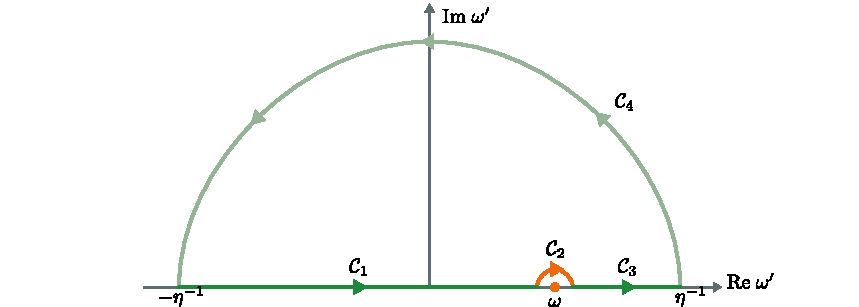
\includegraphics{figs/mt/KK.pdf}
 \caption[Kramers-Kronig contour integral]{ \label{fig:kk}
 \textbf{Kramers-Kronig contour integral.}\small\\
 The contour integral of \eq{kkcontour} can be split into three parts,
 $\mathcal{C}_1 \cup \mathcal{C}_3$ (deep green)
 is the principal value of the integral along the real line;
 $\mathcal{C}_2$ (orange)
 is half the integral around a pole at $\ω$; and
 $\mathcal{C}_4$ (pale green)
 is a contribution that vanishes as the contour limits to infinity.
 }
\end{figure}

A more subtle result that can be derived from the Kramers-Kronig relations is,
that as a function of a complex $\ω$, $\χe(\ω)$ is analytic in the upper
half-plane.
Take the following contour integral,
\begin{equation} \label{eq:kkcontour}
\oint_\mathcal{C}  \d\ω' \:
\frac{\χe(\ω')}{\ω'-\ω}
\;,
\end{equation}
over the closed contour $\mathcal{C}$, where $\mathcal{C}$ is the infinite
semicircle that encloses the upper half-plane, with a infinitesimal semicircular
dent taken out to avoid the pole at $\ω' = \ω$, as shown in \fig{kk},
i.e. $\mathcal{C} = \bigcup_{i=1}^4 \mathcal{C}_i$ with,
\begin{subequations}\subeq
\begin{align}
\mathcal{C}_1 &= [-\η^{-1}, \ω - \η] \\
\mathcal{C}_2 &= \left\{ \ω - \η e^{-i\θ} \middle| \θ \in [0,\π] \right\} \\
\mathcal{C}_3 &= [\ω + \η, \η^{-1}] \\
\mathcal{C}_4 &= \left\{\η^{-1} e^{i\θ} \middle| \θ \in [0,\π] \right\}
\;,
\end{align}
\end{subequations}
in the limit as $\η\→0$.

So long as $\χe(\ω)$ is analytic in the upper half-plane, that is to say there
are no singularities in that region, then \eq{kkcontour} will evaluate to zero.
That is to say,
\begin{equation} \label{eq:kk2}
\int_{\mathcal{C}_1}
+
\int_{\mathcal{C}_2}
+
\int_{\mathcal{C}_3}
+
\int_{\mathcal{C}_4} \d\ω' \:
\frac{\χe(\ω')}{\ω'-\ω}
= 0
\;.
\end{equation}
Contributions from contours 1 and 3 combine to form the principal value of the
integral.
Contour 2 is equal to minus half the residue about the pole
Contour 4 vanishes to zero, which can be understood physically as the
response of a material is unable to match an arbitrarily fast driving term.
This allows the rearrangement of \eq{kk2} as,
\begin{equation}
\PV \int_{-\infty}^{\infty} \d\ω' \:
\frac{\χe(\ω')}{\ω'-\ω}
= \frac{1}{2} 2\π\i \Res\left(\frac{\χe(\ω')}{\ω'-\ω}, \ω\right)
\;.
\end{equation}
which then exactly reproduces \eq{kkComplex}.

This guarantees that the upper half-plane of a causal response function is
analytic, and therefore free of singularities.

\subsection{Drude-Lorentz Model} \label{sec:DrudeLorentz}
One of the most important material models that one can consider is the
Drude-Lorentz model.
It is a causal \cite{Kinsler2011} response that captures the behaviour of most
resonance phenomena.
In its most general terms, it relates the time evolution of $\P$ to a driving
$\E$ field by a second order differential equation:
\begin{equation} \label{eq:tdDL}
\pdd{\P}{t} + \γL\pd{\P}{t} + \ωL^2 \P = \ωp^2 \εf \E
\;,
\end{equation}
where
$\γL$ is a damping term,
$\ωL$ is the restoring force frequency, and
$\ωp$ is the plasma frequency - the coupling strength to the driving $\E$
field.
In frequency domain, one gets,
\begin{equation}
\Ptilde = \εf \frac{\ωp^2}{\ωL^2 - \ω(\ω + i \γL)} \Etilde
\;,
\end{equation}
where the Drude-Lorentz susceptibility can be extracted,
\begin{equation}
\χL(\ω) = \frac{\ωp^2}{\ωL^2 - \ω(\ω + i \γL)}
\;.
\end{equation}
This is analytic in the upper halfplane for $\γL > 0$, and as such obeys the
Kramers-Kronig relations of the previous section.

The origins of a Drude-Lorentz model may vary, and indeed as will be shown
later, a material may host multiple resonances, however, particularly for a
metal, one may explain the origins with a simple model for a free electron gas.
For each electron, let the displacement from its nucleus be given as $\x(\t)$.
A Newtonian force equation can be built from this, using the Lorentz force law,
i.e.,
\begin{equation}
m^* \pdd{\x}{t} = -e \E
\;,
\end{equation}
where $m^*$ is the effective mass of an electron and $e$ is its charge.
Additional forces can be included, such as a collision term proportional to the
velocity and inversely to an average collision time $-\pd{\x}{t}/\τ$.
In this free electron picture, there is no restoring force, though it is
conceivable to add one for electrons bound to a lattice site.
The macroscopic polarisation can be related to these electron displacements, as
each displacement induces an electronic dipole moment, and these can be averaged
to the polarisation by multiplying by the electron number density,
$\P = -e n \x$.
A comparison of terms allows for the mapping,
\begin{equation}
\ωp^2 \→ \frac{n e^2}{m^*} \,,\;
\γ \→ \τ^{-1} \,,\;
\ωL \→ 0
\;.
\end{equation}
This is the Drude model, and with an additional static background permittivity
$\εbg$, it well describes metals.

Real materials typically have multiple resonances, which can be incorporated by
adding multiple Drude-Lorentz resonances,
\begin{equation}
\χ = \sum_i \frac{{\ωp^2}_i}{{\ωL^2}_i - \ω(\ω + i {\γL}_i)}
\;.
\end{equation}
These can have a variety of origins, i.e. in addition to the plasma mode
discussed, rotational modes, electronic transitions, etc.; and indeed the
magnetic response, $\χm$, can also be described as a sum of Drude-Lorentz
resonances.

\section{Transfer Matrix Method} \label{sec:introTMM}
\subsection{Transverse Electric and Transverse Magnetic Solutions}
\label{sec:TETM}
The transverse solutions of \sec{planewaves} can be generalised
to anisotropic media.
Equations~\ref{eq:curlEqs} can be re-written as matrix equations,
\begin{align}
\Etilde = \Z \Zf \Htilde& \\
\Zf \Htilde = \Y \Etilde&
\:,
\end{align}
where $\Z$ and $\Y$ are the impedance and admittance tensors, respectively,
defined as,
\begin{align}
\Z = -\frac{c}{\ω} \εtens^{-1} \crossmat{\Q}& \\
\Y = \frac{c}{\ω} \μtens^{-1} \crossmat{\Q}&
\:,
\end{align}
with $\crossmat{\Q}$ defined as the cross product with $\Q$ expressed as a
matrix.
This allows the electric and magnetic fields to be written as an eigenvalue
equation,
\begin{align}
\Etilde &= \Z\Y \Etilde \\
\Zf \Htilde &= \Y\Z \Zf \Htilde
\:.
\end{align}
The matrix $\Z\Y$ (and $\Y\Z$) has one zero eigenvalue, and by solving for the
other two to be equal to one will give the dispersion relation for two
independent planewave solutions.
The eigenvectors will determine the field polarisation for each solution.

Consider a medium with non-singular permittivity and permeability that are
simultaneously diagonalisable, i.e.,
$\εtens = \diag(\εx, \εy, \εz)$ and $\μtens = \diag(\μx, \μy, \μz)$
in this coordinate system.
Further assume that the wave propagates in a plane normal to the $y$-direction,
i.e. $\Q = (q, 0, \κ)^\TP$.
The resulting two solutions become the basis for
\emph{transverse electric} (\TE) modes,
\begin{subequations}\subeq
\begin{align}\label{eq:TEdisp}
\μx \μz \εy \frac{\ω^2}{\c^2} &- \μx {q}^{2} - \μz {"\κ}^2 = 0 \\
\Etilde &= \EtildeAbs  \left(0, 1, 0\right)^\TP \\
\Zf\Htilde &= \EtildeAbs
\left(-\frac{\c \κ}{\μx \ω}, 0, \frac{\c q}{\μz \ω}\right)^\TP
\;,
\end{align}
\end{subequations}
and \emph{transverse magnetic} (\TM) modes  that will be discussed later in this
section,
\begin{subequations}\subeq
\begin{align}\label{eq:TMdisp}
\εx \εz \μy \frac{\ω^2}{\c^2} &- \εx {q}^{2} - \εz {"\κ}^2 = 0 \\
\Etilde &= \EtildeAbs
\left(1, 0, -\frac{\εx q}{\εz \κ}\right)^\TP \\
\Zf\Htilde &= \EtildeAbs  \left(0, \frac{\εx \ω}{\c \κ}, 0\right)^\TP
\;,
\end{align}
\end{subequations}

\subsection{Planar Boundaries}
Until now we have considered electromagnetic fields in a homogeneous space,
however there is a lot of interesting physics to be found at the boundaries
between different media, and indeed the majority of this thesis considers
surface phenomena.

Consider two infinite half-spaces divided by a planar boundary at $z = 0$.
Let each half-space be filled with a medium, characterised by permittivity and
permeability $\εtens$ and $\μtens$ as described above.
The solutions in each half-space can be assumed to be the same as
those in the homogeneous case for each medium, i.e. planewaves.\footnote{
Strictly, this is only true if the media are local in the direction
normal to the interface.}

It then becomes a question to derive the \emph{boundary equations}
which knit together the solutions at the boundary of the spaces.
To start one takes the Macroscopic Maxwell's Equations, \eq{macME},
and applies Gauss' and Stokes' theorems, to yield their integral form,
\begin{subequations}\subeq
\begin{align}
\oiint_{\partial V} \D \cdot \dS &= \iiint_V \ρext \dV
\\
\oiint_{\partial V} \B \cdot \dS &= 0
\\
\oint_{\partial \σ} \E \cdot \dl &=
 - \pd{}{t} \iint_{\σ} \B \cdot \dσ
\\
\oint_{\partial \σ} \H \cdot \dl &= \iint_{\σ} \Jext \cdot \dσ
 + \pd{}{t} \iint_{\σ} \D \cdot \dσ
\;,
\end{align}
\end{subequations}
Allowing for the possibility of surface charges and currents,
$\ρext = \ρs \δ(z)$ and $\Jext = \Js \δ(z)$,
and taking the volume of integration, $V$, to be a cube of arbitrary $x$,$y$
dimension, but infinitesimally thin in $z$ and straddling the boundary plane,
then,
\begin{subequations}\subeq
\begin{align}
(\Dme_2 - \Dme_1) \cdot \ez &= \ρs \\
(\Bme_2 - \Bme_1) \cdot \ez &= 0
\;.
\end{align}
The surface of integration, $\σ$, is a plane parallel to $z$ and either $x$ or
$y$, again infinitesimal in $z$, this gives the further relations,
\begin{align}
\ez \times (\Eme_2 - \Eme_1) &= 0 \\
\ez \times (\Hme_2 - \Hme_1) &= \Js
\;.
\end{align}
\end{subequations}
Where subscripts 1 and 2 refer to the values of the fields just below and just
above of the interface.

For the planewaves to maintain continuity between each half-space,
they must be of the same frequency, and have the same component of wavevector
parallel to the surface.
Considering the space-time domain solution of a single frequency component,
this restricts the value of the perpendicular component of the wavevector to be
determined by \eqs{TEdisp}{TMdisp}, for which there are two solutions, since
they are equations in $\κ^2$.
The solution in each space is given as,
\begin{equation}\label{eq:EFwBw}
\E =
\begin{cases}
\E_1^+ e^{\i(q x + \κ_1 z - \ω \t)} +
\E_1^- e^{\i(q x - \κ_1 z - \ω \t)} + \cc
& : z < 0
\\
\E_2^+ e^{\i(q x + \κ_2 z - \ω \t)} +
\E_2^- e^{\i(q x - \κ_2 z - \ω \t)} + \cc
& : z > 0
\end{cases}
\;,
\end{equation}
with equivalent solutions for $\H$, $\B$, and $\D$.
The surface charges and currents can be included with the additional
constitutive relation, defining the surface conductivity $\σs$,
\begin{subequations}\subeq
\begin{align}
\Js &= \σs(\q, \ω) \E^\shortparallel (z=0) \\
\ρs &= \σs(\q, \ω) \q \cdot \E^\shortparallel (z=0) / \ω
\;,
\end{align}
\end{subequations}
where the parallel symbol on $\E^\shortparallel$ indicates the $z$ component of
that vector is set to zero, and $\q$ is the $x,y$ plane projection of $\Q$.

To proceed, one needs to consider the \TE and \TM solutions in turn and apply
the boundary value conditions for $z=0$.

For the \TE solution, the non-zero $\E$ and $\H$ field components are $E_y$,
$H_x$, and $H_z$. This though is overdetermined, with
$\Zf H_z = q \c / (\ω \μpar_z)  E_y$.
The boundary value problem can be expressed as a matrix\footnote{
In order to keep $E_y$, $H_x$, and $z$ as a right handed triplet (and for
symmetry with the \TM matrices) the matrix is expressed for (a negative) $-H_x$.
},
\begin{subequations}\subeq
\begin{equation}
\begin{pmatrix}
E_{y2} \\
-\Zf H_{x2}
\end{pmatrix}
=
\underbrace{
\begin{pmatrix}
1 & 0 \\
-\Zf \σs & 1
\end{pmatrix}
}_{\v{S}^\TE}
\begin{pmatrix}
E_{y1} \\
-\Zf H_{x1}
\end{pmatrix}
\;,
\end{equation}
where it can be verified that this also continues the auxiliary fields in the
correct manner.
One may determine the coefficients of the forward and backward propagating waves
in \eq{EFwBw} by expressing it in matrix form for $\x=0$, $t=0$,
\begin{equation}
\begin{pmatrix}
E_{yi} \\
-\Zf H_{xi}
\end{pmatrix}
=
\underbrace{
\begin{pmatrix}
1 & 1 \\
1/\uTE_i & -1/\uTE_i
\end{pmatrix}
}_{\v{U}^\TE}
\begin{pmatrix}
A^+_i \\
A^-_i
\end{pmatrix}
\;,
\end{equation}
with $\uTE_i = \μ_{x i} \ω/(\c \κ_i)$, is the angle dependent\footnote{
For normal incidence, $q=0$, the impedances take the more familiar form,
$\uTE = \sqrt{\μ_x / \ε_y}$ and $\uTM = \sqrt{\μ_y / \ε_x}$.
} impedance,
and $A^\pm_i = \E^\pm_i \cdot \ey$.

The fields can then be calculated at any $z$ coordinate by propagating the
forward and backward components,
\begin{equation}
\left.
\begin{pmatrix}
A^+_{i} \\
A^-_{i}
\end{pmatrix}
\right|_{z}
=
\underbrace{
\begin{pmatrix}
e^{\i \κ_i (z - z')} & 0 \\
0 & e^{-\i \κ_i (z - z')}
\end{pmatrix}
}_{\v{T}}
\left.
\begin{pmatrix}
A^+_{i} \\
A^-_{i}
\end{pmatrix}
\right|_{z'}
\;,
\end{equation}
and of course, at any $x$ and $\t$ by multiplication of $e^{i(q x - \ω \t)}$.
\end{subequations}

The equivalent \TM transfer matrices are given as,
\begin{subequations}\subeq
\begin{align}
\begin{pmatrix}
 E_{x2} \\
 \Zf H_{y2}
\end{pmatrix}
&=
\underbrace{
\begin{pmatrix}
 1 & 0 \\
 -\Zf \σs & 1
\end{pmatrix}
}_{\v{S}^\TM}
\begin{pmatrix}
 E_{x1} \\
 \Zf H_{y1}
\end{pmatrix}
\\
 \begin{pmatrix}
 E_{x i} \\
\Zf H_{y i}
\end{pmatrix}
&=
\underbrace{
\begin{pmatrix}
 1 & 1 \\
 1/\uTM_i & -1/\uTM_i
\end{pmatrix}
}_{\v{U}^\TM}
\begin{pmatrix}
 A^+_i \\
 A^-_i
\end{pmatrix}
\\
\left.
\begin{pmatrix}
 A^+_{i} \\
 A^-_{i}
\end{pmatrix}
\right|_{z}
&=
\underbrace{
\begin{pmatrix}
 e^{\i \κ_i (z - z')} & 0 \\
 0 & e^{-\i \κ_i (z - z')}
\end{pmatrix}
}_{\v{T}}
\left.
\begin{pmatrix}
 A^+_{i} \\
 A^-_{i}
\end{pmatrix}
\right|_{z'}
\;,
\end{align}
\end{subequations}
with $\uTM_i = \c \κ_i / (\εpar_{x i} \ω)$.
These are the matrices of the \emph{transfer matrix method} (\tmm).
The matrices, $\v{S}$, $\v{U}$, and $\v{T}$, in both the \TE and \TM
case, are assigned respectively such that $\v{S}$ continues electric and
magnetic fields from one medium over an interface into another;
$\v{U}$ converts from the basis of forward and backward travelling waves to
electric and magnetic field components;
and $\v{T}$ propagates forward and backward travelling waves from a point $z'$
to a point $z$.

\subsection{Stratified Media} \label{sec:stratmed}

\begin{figure}
 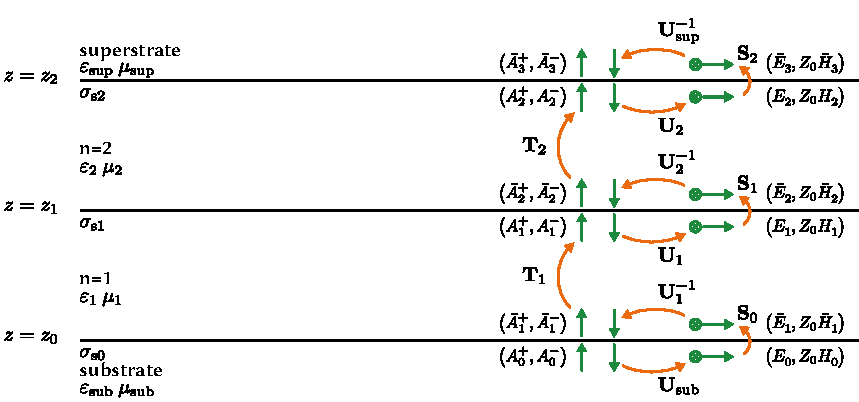
\includegraphics{figs/mt/TMM.pdf}
 \caption[Schematic of the transfer matrix method]{\label{fig:TMM}
 \textbf{Schematic of the transfer matrix method.}\small\\
 Fields (green arrows) are operated on by matrix transformations (orange
 arrows).
 The forward and backward components at the top of substrate layer
 $(A_0^+,A_0^-)$ are transferred through the stack to forward and backward
 components at the bottom of the superstrate layer $(\bar{A}_3^+,\bar{A}_3^-)$.
 Fields move between bases of forward and backward waves (↑ ↓) and
 electric and magnetic components (⊗ →).
 }
\end{figure}

Up until now, this matrix description can be at best described as book-keeping.
Its utility will become clear when generalising to stratified media.
Consider a stack of $N$ planar slabs on a substrate as in \fig{TMM}, each with
its own material properties.
Let the top interface of the $i\th$ slab be at $z_i$, vector
components with that label, e.g. $A^\pm_i$, be measured from there, i.e. just
below the top interface in that layer.
Starting in the forward and backward basis, one may
use the transfer matrices to propagate through the stack from the one layer to
the next.
\begin{equation}
\begin{pmatrix}
A^+_{i+1} \\
A^-_{i+1}
\end{pmatrix}
=
\v{T}_{i+1} \v{U}_{i+1}^{-1} \v{S}_i \v{U}_i
\begin{pmatrix}
A^+_{i} \\
A^-_{i}
\end{pmatrix}
\;.
\end{equation}
The exception to this being the superstrate, the $(N+1)\th$ layer,
which by definition does not have a top interface.
As such $E^\pm_\sup$ is defined specially as the forward and backward
components just above the top interface of the $N\th$ layer, i.e.,
\begin{equation}
\begin{pmatrix}
A^+_\sup \\
A^-_\sup
\end{pmatrix}
=
\v{U}_\sup^{-1} \v{S}_N \v{U}_N
\begin{pmatrix}
A^+_{N} \\
A^-_{N}
\end{pmatrix}
\;.
\end{equation}
The full transfer matrix $\Mtr$ is given as the product of each layer hop,
\begin{equation}
\Mtr = \v{U}_\sup^{-1} \v{S}_N \v{U}_N \dotsm \v{T}_{1} \v{U}_{1}^{-1}
\v{S}_0 \v{U}_\sub
\;.
\end{equation}
Terms with similar indices can be grouped to give a matrix for each layer
\footnote{
Thin film (non-magnetic) layers with thickness $\δ \→ 0$ can be approximated as
$\v{M} \approx \v{S}$, with $\Zf\σs \→ -i\δ(\ω/c) \ε_x$ for \TM and $\Zf\σs \→
-i\δ(\ω/c) \ε_y$ for \TE solutions.
},
\begin{equation}
\v{M}_i = \v{U}_i \v{T}_{i} \v{U}_{i}^{-1}
\;,
\end{equation}
such that the transfer matrix for the whole stack is,
\begin{equation}
\Mtr =
\v{U}_\sup^{-1}
\left( \prod_{i=N}^1 \v{S}_i \v{M}_i \right)
\v{S}_0 \v{U}_\sub
\;,
\end{equation}
noting the reverse order on the product.

The matrix $\Mtr$ maps forward and backward travelling waves in the substrate to
forward and backward waves in the superstrate.
This can be used to calculate reflection and transmission spectra.
Assume a plane wave incident in the superstrate,
this will both reflect at the surface and transmit into the substrate.
This can be codified as a matrix equation, with the assumption that there is no
incoming wave from the substrate,
\begin{equation}
\begin{pmatrix}
r \\ 1
\end{pmatrix}
=
\Mtr
\begin{pmatrix}
0 \\ t
\end{pmatrix}
\;,
\end{equation}
where $1$, $r$, $t$ are the coefficients of the incoming, reflected, and
transmitted components, respectively, of the $E$ field parallel to the stack.
This is solved as,
\begin{subequations}\subeq
\begin{align} \label{eq:reflCoeffs}
t &= (\Mtr_{2 2})^{-1} \\
r &= (\Mtr_{1 2}) / (\Mtr_{2 2})
\;.
\end{align}
\end{subequations}

The coefficients $r$ and $t$ can be used to determine the power flows by the
introduction of the Poynting vector,
\begin{equation}
\S(\x, t) = \E(\x,t) \× \H(\x,t)
\;,
\end{equation}
which is the flux vector of electromagnetic power \cite{Griffiths2013}.
Because it is the product of fields, it is strictly speaking defined only in
space-time domain, however for quasi-monochromatic fields the time-averaged
Poynting vector can be defined as:
\begin{equation}
\left\langle \S \right\rangle = \frac{1}{2} \Re \left(
\E \× \H^*
\right)
\;.
\end{equation}
The component normal to the stacking is of most interest, and in both the \TM
and \TE case, this can be calculated in each layer as,
\begin{equation}
\left\langle \S \right\rangle_z = \Re \frac{1}{2 Z_i \Zf} \left(
|A^+_i|^2 - |A^-_i|^2
\right)
+ \Im \frac{1}{Z_i \Zf} \Im \left( A_i^{+*} A_i^- \right)
\;.
\end{equation}
The first term is power transferred in propagating fields, while the last term
describes power in evanescent fields.

For propagating waves incident in a lossless upper half-plane, the ratio of
reflected and transmitted power flows to the incident power is calculated as,
\begin{subequations}\subeq
\begin{align}
R &= \left.
 \Re \frac{1}{2 Z_\sup \Zf} |A^+_\sup|^2
\middle/
 \Re \frac{1}{2 Z_\sup \Zf} |A^-_\sup|^2
\right.
\\ 
T &= \left.
 \Re \frac{1}{2 Z_\sub \Zf} |A^-_\sub|^2
\middle/
 \Re \frac{1}{2 Z_\sup \Zf} |A^-_\sup|^2
\right.
\;.
\end{align}
\end{subequations}
In in terms of the coefficients of \eq{reflCoeffs}, this reads,
\begin{subequations}\subeq
\begin{align}
R &= |r|^2
\\ 
T &= \frac{\Re Z_\sub^{-1}}{\Re Z_\sup^{-1}}|t|^2
\;.
\end{align}
\end{subequations}

One point has been so far glossed over: the branch of the square
root of $\κ^2$.
Both positive and negative solutions are included, but to identify one or the
other as forward or backward travelling waves, one must chose $\κ$ such that
$\Re \κ > 0$ in the superstrate.
In the substrate the situation is more complicated, since the waves may be
either propagating or evanescent here.
If $\κ$ is real, pick the positive root,
but if it is complex or imaginary, it must be picked such that $\Im \κ > 0$,
This will guarantee that fields exponentially decay from the surface rather
than diverging.

\subsection{Surface Plasmon Polariton}

With the transfer matrix, one is also able to calculate the bound modes of a
system.
These are the eigenmodes of the system which have non-zero fields for a zero
driving field, i.e.,
\begin{equation}
\begin{pmatrix}
A^+_\sup \\ 0
\end{pmatrix}
=
\Mtr
\begin{pmatrix}
0 \\ A^-_\sub
\end{pmatrix}
\;,
\end{equation}
with the prescription that $\Im \κ > 0$ in both the super- and substrate, such
that fields on both sides decay away to infinity.
This yields the condition that $\Mtr_{2 2} = 0$ for bound modes.
In general this is satisfied for either one of the frequency $\ω$ or wavevector
$q$ being a complex number, with the other remaining real.

Here the example of the surface plasmon polariton (\spp) is considered, a mode
that exists on the interface between a metal and an insulator, where charge
carriers on the metal's surface couples to the electric field.
\textsc{Spp}s are of interest because, as will be shown, they permit field
solutions which extend beyond the diffraction limit, allowing for high
confinement of electromagnetic energy and large field enhancement at the
interface.

Consider a metal substrate and dielectric superstrate, the metal
characterised by a dispersive permittivity $\εpar(\ω)$ and the dielectric by a
static constant $\εD$.
Both layers are non-magnetic, $\μpar = 1$, and there is no external surface
conductivity $\σs = 0$.
S\textsc{pp} modes are \TM in nature, so we shall only seek these solutions.
It can be shown that \TE \spp solutions do not exist \cite{book:Maier}.

In this case the transfer matrix is given as,
\begin{subequations}\subeq
\begin{align}
\Mtr &= \v{U}_\sup^{-1} \v{U}_\sub
\\
 &=
\frac{1}{2}
\begin{pmatrix}
 1 & \frac{\c \κ_\sup}{\εD \ω} \\
 1 & -\frac{\c \κ_\sup}{\εD \ω}
\end{pmatrix}
\begin{pmatrix}
 1 & 1 \\
 \frac{\εpar(\ω) \ω}{\c \κ_\sub} & -\frac{\εpar(\ω)  \ω}{\c \κ_\sub}
\end{pmatrix}
\;,
\end{align}
\end{subequations} 
which gives the \spp condition,
\begin{equation}
\Mtr_{2 2} = \frac{1}{2}
\left( \frac{\c \κ_\sup}{\εD \ω} \frac{\εpar(\ω) \ω}{\c \κ_\sub} + 1 \right)
 = 0
\end{equation}
\begin{equation}
\frac{\εpar(\ω)}{\εD} + \frac{\κ_\sub}{\κ_\sup} = 0
\;.
\end{equation}
One can see that for this equation to have solutions, given $\εD > 0$ and $\Im\κ
> 0$, then it must hold that $\Re \εpar(\ω) < 0$, which is characteristic of
metals for frequencies below their plasma frequency.

For a lossless Drude metal, i.e. $\εpar(\ω) = \εinf- (\ωp/\ω)^2$, an analytical
solution exists,
\begin{equation}
q^{2} = \εD \left(\frac{\ω}{\c}\right)^2
\frac{
 \εinf \ω^2 - (\εD + \εinf) \ωsp^2
}{
 (\εD + \εinf)(\ω^2 - \ωsp^2)
}
\;,
\end{equation}
where $\ωsp = \ωp / \sqrt{\εD + \εinf}$, is the \emph{surface plasmon
frequency}.

For small wavevectors, the dispersion relation becomes
$\ω \→ q c / \sqrt{\εD}$, where it follows the dielectric medium
lightline.
As the wavevector increases, the curve shall become shallower than the light
line and as $q\→\infty$, the dispersion relation tends to the limiting value
$\ω \→ \ωsp$.
Here the \spp transitions between being photonic in character to becoming like a
\emph{surface plasmon}, where the field limits to being entirely confined to
the surface.
The diffraction limit is surpassed here as an arbitrarily large wavevector range
is supported at a small frequency range, in the limit of no loss.

In this thesis, multi-layer structures will be considered that support hybrid
\spp modes about one or multiple material interfaces.
In general, analytical dispersion relation solutions do not exist, but rather
solutions for $\Mtr_{2 2}(\q, \ω) = 0$ are found implicitly, using a
root-finding algorithm.

\section{Finite Difference Time Domain} \label{sec:fdtd}
\begin{figure}
 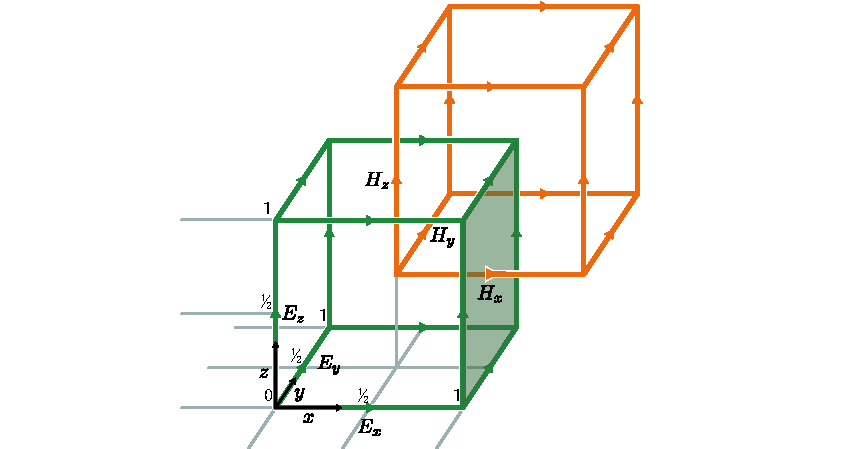
\includegraphics{figs/mt/FDTD.pdf}
 \caption[Schematic of \fdtd Yee cell]{ \label{fig:FDTD}
 \textbf{Schematic of \fdtd Yee cell.}
 Electric (green) and magnetic (orange) field grids.
 They are shifted half a step from each other, forming an interlocking link.
 Each field line passes through the centre of a square formed from lines of the
 other field, e.g. $H_x$ here passes through the centre of the highlighted
 $E$-field face, where the finite difference $\curl \E$ is defined.
 }
\end{figure}

The real world exists in time domain; whereas the frequency domain is
mathematically complementary, the purpose of calculations done in it must
ultimately be to get a handle on the time evolution of a system.
As the complexity of a system increases, analytic methods begin to get less and
less tractable.
In order to complement such techniques, numerical simulations may be employed.
In this thesis, the \emph{finite difference time domain}
(\fdtd) method \cite{Yee1966,Taflove1995} will be used.

In \fdtd, the goal is to solve Maxwell's equations for successive instants in
time over a discretised lattice.
This is approached by taking the curl equations, and making the time derivatives
of the fields the subject.
Making the assumption that there are no external sources,
\begin{subequations}\subeq
\begin{align}
\pd{\E}{\t}  &= \frac{1}{\εf} \left( \curl \H - \pd{\P}{\t} \right) 
\\
\pd{\H}{\t}  &= -\frac{1}{\μf} \left( \curl \E -\pd{\M}{\t} \right) 
\;.
\end{align}
\end{subequations}
Now, space and time are discretised as
$(t, x, y, z) \→ ( n\Δt, i\Δx, j\Δx, k\Δx )$ and
derivatives are turned into finite differences, i.e.,
\begin{equation}
\pd{\E}{t}(\x, t) \→ \frac{\E^{n+1}_{i, j, k} - \E^n_{i, j, k}}{\Δt}
\;.
\end{equation}
Strictly, the above is a central difference and approximates the time derivative
at a time $(n+1/2)\Δt$.
Therefore the corresponding right-hand-side terms must be evaluated at
this time.
The curl operator is handled similarly,
\begin{equation}
\curl \E(\x, t)|_x \→ \frac{E_z|^n_{i, j+1, k} - E_z|^n_{i, j, k}}{\Δx} -
\frac{E_y|^n_{i, j, k+1} - E_y|^n_{i, j, k}}{\Δx} \;.
\end{equation}
In order to make best of this central difference, the lattice is arranged as
a Yee grid \cite{Yee1966}, where fields are stored separately by component and
$\E$ and $\P$ fields are specified on integer time coordinates, whereas $\H$ and
$\M$ are specified on half integer time coordinates.
The lattice coordinates are more complicated, for $\E$, components are stored
at half-integer coordinates in their own direction and at integer coordinates
otherwise.
This is the opposite for the $\H$ field, as illustrated in
\fig{FDTD}.
From here, one can write the \emph{update equations},
\begin{subequations}\subeq
\begin{align}
E_x|^{n+1}_{i+\½, j, k} &= E_x|^n_{i+\½, j, k}
- \εf^{-1} P_x|^{n+1}_{i+\½, j, k} + \εf^{-1} P_x|^n_{i+\½, j, k}
\\ \nonumber
&+ \frac{c\Δt}{\Δx}
\left(
  \Zf H_z|^{n+\½}_{i+\½, j+\½, k} - \Zf H_z|^{n+\½}_{i+\½, j-\½, k}
\right)
\\ \nonumber
&- \frac{c\Δt}{\Δx}
\left(
  \Zf H_y|^{n+\½}_{i+\½, j, k+\½} - \Zf H_y|^{n+\½}_{i+\½, j, k-\½}
\right)
\\
\Zf H_x|^{n+\½}_{i, j+\½, k+\½} &= \Zf H_x|^{n-\½}_{i, j+\½, k+\½}
+
c M_x|^{n+\½}_{i, j+\½, k+\½} - c M_x|^{n-\½}_{i, j+\½, k+\½}
\\ \nonumber
&+ \frac{c\Δt}{\Δx}
\left(
  E_z|^{n}_{i, j+1, k+\½} - E_z|^{n}_{i, j, k+\½}
\right)
\\ \nonumber
&- \frac{c\Δt}{\Δx}
\left(
  E_y|^{n}_{i, j+\½, k+1} - E_y|^{n}_{i, j+\½, k}
\right)
\;,
\end{align}
\end{subequations}
with corresponding equations for the omitted components.

With the update equations of the primary fields determined, it remains to
describe how the auxiliary fields update.
In general, the constitutive equations are functionals of all past values of all
fields, as described in \sec{constitutive} and \sec{KKrels}, though this would
prove tricky to directly implement.
In practice, material responses can be cast in terms of a finite difference if
they can be expressed in terms of a temporal differential equation.
This lends the Drude-Lorentz model of \sec{DrudeLorentz} well to inclusion
within \fdtd, though it's update equations and how to incorporate them are
beyond the scope of this thesis.

The \fdtd algorithm therefore proceeds by iterating over updating in order the
$\E$ field, $\M$ field, $\H$ field, and $\P$ field over all space for each
timestep.

There are limitations to \fdtd.
Its staggered grid structure means that material interfaces are not sharply
defined, and any curvature on an interface will also experience a staircasing
effect that can lead to spurious hot-spots especially in plasmonic structures
where geometric effects play a key role.
The grid is also regular, which is to say it can not be adaptively refined in
areas of interest, rather all points must be simulated to the same resolution.
This adds to the numerical load, as the smallest wavelength component of the
fields, as well as the smallest geometrical features must be provided with
sufficient resolution.
This is again especially relevant in plasmonics, where field confinement is a
feature.

Because of its nature as a full wave time domain solver, \fdtd can often be the
final say on a theoretical investigation.
Short of doing a real-world experiment, \fdtd numerical simulations find their
utility as a heavy-duty tool.
That is, the Maxwell's equations are solved at every discretised point in space,
so it is often slower and more cumbersome, but can as a result of the inherent
thoroughness produce results for questions that other techniques are unable to.

\section{Evolutionary Algorithm} \label{sec:EA}

\begin{figure}
 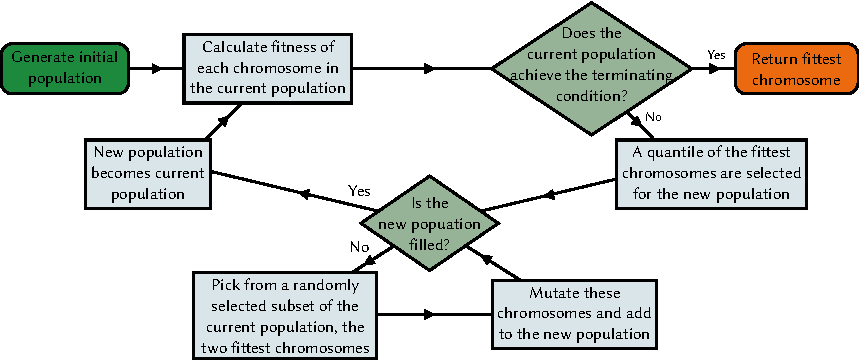
\includegraphics{figs/mt/Flow.pdf}
 \caption[Evolutionary algorithm flowchart]{\small \label{fig:flow}
 \textbf{Evolutionary algorithm flowchart.}
 }
\end{figure}

For a planar stratified structure whose properties can be determined by a
transfer matrix method, one may wish to optimise some aspect of its response to
electromagnetic radiation.
This may be in the dispersion relation of bound modes or in the transmission and
reflection spectra.
For example, to prescribe the frequency of a bound mode, or a
reflection peak; or set whether there is only a single mode or
many modes within a frequency range; or control the amplitude and phase response
to an incoming wavepacket.
These properties are entirely determined by the composition of the structure,
however it often not obvious how changes in the structure lead to changes in the
response.

The structures to be considered can be described by a finite number of numeric
or discrete parameters, i.e. for each layer: the thickness of the layer, the
material model to use, and the parameters of that model.
This is well suited to optimisation using an \emph{evolutionary algorithm}
(\ea) \cite{Spears2000}.

In brief, an \ea operates by storing multiple copies of these parameter sets,
perturbing the values of the parameters randomly, ordering the sets by how the
system they describe performs against a fitness metric, and keeping only the
best variants to the next round.

More fully, in the language of an \ea, this would be to say that a
\emph{population} of \emph{chromosomes} is kept, and on each iteration of the
algorithm, new chromosomes are generated from \emph{mutations} of the current
ones, the next generation population is filled by \emph{selection} of these
chromosomes by a \emph{fitness function}.
The goal of the \ea is to find a chromosome which extremises the fitness
function globally, and as such an \ea is most suitable when the evaluation of
the fitness function can be performed relatively quickly as a large number of
members of the state space must be evaluated and compared.

A chromosome is simply the set of parameters which describes a system, i.e.
a list of numbers or discrete option values.
They are atomic entities, independent of other chromosomes.
Each chromosome may have its fitness function evaluated to determine how
suitable its corresponding physical system is to a problem.

Each iteration of the \ea holds a set of chromosomes, ordered by their fitness
function, known as a \emph{population}.
The first generation is seeded population either
with randomly generated structures, or structures that have been tuned by hand,
perhaps by approximative theoretical methods.
Populations of subsequent generations are constructed by firstly taking a small
quantile of the fittest chromosomes from the previous iteration, with the
remaining places filled with \emph{mutations} of chromosomes selected from the
previous set.
The progress of the algorithm can be tracked by examining the fittest chromosome
at the end of each iteration.
At the end of each iteration, a \emph{terminating condition} is evaluated, which
determines if the algorithm should stop, returning the fittest chromosome, e.g.
if the best structure in the population is within a defined tolerance of the
target output, or if a set number of iterations have elapsed.
If the terminating condition is not met, then the algorithm continues for
another iteration.
The operation of the \ea is described as a flowchart in \fig{flow}.

The mutation process generates a new chromosome by randomly perturbing the
values of parameters of a parent chromosome.
It is by mutation that the state space of chromosomes is mapped.

For the layered structures considered here, the mutation process will perturb
both the properties of the layers themselves, and the relationship between
layers.
Numeric parameters, such as layer thicknesses and those used in material
models are perturbed by a Gaussian random variable, and the discrete
parameters, such as the layer model, can be randomly selected from a list.
Typically only one or few parameters will be changed in each mutation.
The parameters of the layers themselves don't sit in isolation.
The number of layers in these structures is variable and mutation
allows for adding or removing of layers or indeed swapping the order of layers
and shifting the boundary between adjacent layers.

Whereas the \ea is widely applicable to problems in nano-optics,
the fitness function is not general and has to be constructed for each problem
based on what characteristics are to be selected for.
In \sec{SLOptimisation} a fitness function will be defined for structures that
hold light in a bound mode at zero group velocity, seeking to reduce the
dispersion of a wavepacket propagating in the structure.
